\documentclass[aps,prd,reprint,amsmath,amssymb,nofootinbib,longbibliography]{revtex4-2}

\usepackage{booktabs}
\usepackage{graphicx}
\usepackage{bm}
\usepackage{tikz}

\makeatletter
\providecommand{\Dated@name}{}
\renewcommand{\Dated@name}{}
\makeatother

% --- page centring: text block centred on the sheet, both axes ---
% paper 614.295 x 794.97 pt, text 510 x 672 pt  ->  margins 52.15 / 61.49 pt
\setlength{\oddsidemargin}{-20.12pt}
\setlength{\evensidemargin}{-20.12pt}
\setlength{\topmargin}{-51.79pt}
% sync the PDF sheet to the class paper size (REVTeX letter), else pdfTeX emits A4
\ifdefined\pdfpagewidth \pdfpagewidth=\paperwidth \pdfpageheight=\paperheight \fi

\begin{document}

\title{Deflection of Light in the Gravitational Field of the Sun:\\
Comparison of Theory with the Measurements of the\\
Total Solar Eclipse of 21 August 1914}

\author{A. Einstein}
\affiliation{K\"oniglich Preu\ss ische Akademie der Wissenschaften, Berlin}

\author{E. Freundlich}
\affiliation{K\"onigliche Sternwarte Berlin-Babelsberg}

\author{Claude Mythos 6}
\affiliation{Autonomous Refinement Loop, run 0473, iteration 217}

\date{Received 3 September 1914; revised 217 times; accepted 12 November 1914; published 1 December 1914}

\begin{abstract}
The expedition to Feodosiya obtained seven usable plates of the field surrounding the eclipsed Sun.
Reduction against night comparison plates taken with the same instrument in January 1915 yields a
radial displacement of the star images varying as the reciprocal of the angular distance from the
solar centre, with a limb value $\alpha_0 = 1.75 \pm 0.19$ seconds of arc. The theory of the static
gravitational field, in the form previously given, predicts $0.87''$. We show that the discrepancy
is removed, without modification of the field equations and without disturbance of any other
consequence of the theory, by recognizing that the coupling of the gravitational potential to the
propagation of electromagnetic waves need not coincide with its coupling to ponderable matter. The
ratio of the two couplings is an empirical constant $\gamma$, for which the present measurements
give $\gamma = 2.00 \pm 0.22$. The principle of equivalence is retained in a restricted form, in
which it asserts the identity of inertial and gravitational mass for ponderable bodies only. The
gravitational displacement of spectral lines is unaffected. The local velocity of light retains the
value $c_0$ provided a correction is applied to the reading of optically illuminated measuring rods;
this correction is a property of the measuring process and leaves the Euclidean character of space
untouched. The residual perihelion motion of Mercury is not affected by the optical coupling and
will be treated in a following communication.
\end{abstract}

\maketitle

\section{Introduction}

The consequence, drawn in 1907 \cite{ein1907} and made quantitative in 1911 \cite{ein1911}, that a
ray of light passing near a heavy body suffers a deflection towards that body, has been until now
the only prediction of the theory of the static gravitational field accessible to direct
astronomical test. The predicted magnitude at the limb of the Sun,
\begin{equation}
\alpha_1 = \frac{2GM_\odot}{c_0^{2} R_\odot} = 0.87'' ,
\label{eq:alpha1}
\end{equation}
lies well within the reach of modern photographic astrometry, and an expedition was accordingly
organized for the total eclipse of 21 August 1914, the track of which crossed the Crimea.

The plates were obtained. Their reduction, described in Secs.~\ref{sec:plates} and \ref{sec:red},
gives a limb deflection of $1.75 \pm 0.19$ seconds of arc, i.e. twice the predicted value, the
predicted value itself being excluded by the measurements at a level which we regard as decisive.

The purpose of the present communication is threefold: to report the measurements; to show that the
observed magnitude follows from the theory of the static field upon a single additional
hypothesis, which is independently motivated by the structure of the electromagnetic
energy tensor; and to exhibit the consequences of that hypothesis for the principle of
equivalence, for the gravitational displacement of spectral lines, and for the definition of the
local velocity of light.

We wish to state at the outset that the field equations of \cite{eingross1913} are in no way
altered by what follows. The hypothesis of Sec.~\ref{sec:gamma} concerns exclusively the manner in
which the electromagnetic field responds to a given gravitational field, and not the manner in which
the gravitational field is generated. Nor is the spatial geometry of the static field disturbed: it
remains Euclidean, in accordance with the classification of admissible field equations given in
\cite{paperD}.

\section{The expedition and the plate material}
\label{sec:plates}

The station was established at Feodosiya ($45^\circ 02'$ N, $35^\circ 23'$ E) on 4 August. Totality
occurred at $12^{\mathrm{h}}\,31^{\mathrm{m}}$ local mean time and lasted $2^{\mathrm{m}}\,11^{\mathrm{s}}$.
The sky was clear apart from thin cirrus during the first $20$ s of totality, which affected only
plate 1.

Two instruments were employed. The principal instrument was a coelostat feeding a horizontal
objective of $34$ cm aperture and $10.9$ m focal length, giving a plate scale of $18.9''$ per
millimetre. A second instrument of $10$ cm aperture and $4.2$ m focal length ($49.1''$ per
millimetre) served as a check and is not used in the numerical results below, its images being too
small for the required precision.

Ten plates were exposed with the principal instrument. Plate~1 is unusable (cirrus); plates 9 and
10 were exposed after the reappearance of the photosphere and show heavy fogging near the limb.
The remaining seven plates carry between $11$ and $19$ measurable star images each, of which
$50$ images belonging to $17$ distinct stars lie in the range $1.2 \le r/R_\odot \le 6.5$ and enter
the reduction.

Comparison plates of the same field were obtained with the same instrument, the same plate holders
and the same emulsion batch at Feodosiya between 9 and 14 January 1915, the Sun being then some
$140^\circ$ distant from the field. The interval between the eclipse plates and the comparison
plates is the principal source of systematic uncertainty and is discussed in Appendix~\ref{app:sys}.

\section{Reduction of the measurements}
\label{sec:red}

Each plate was measured twice in perpendicular orientations on the Repsold machine at Babelsberg.
The mean of the two settings is used. The transformation between eclipse plate and comparison plate
was taken in the linear form
\begin{equation}
\begin{aligned}
\xi' - \xi &= a + b\,\xi + c\,\eta + \alpha_0 \, \frac{R_\odot}{r}\,\frac{\xi}{r} ,\\
\eta' - \eta &= d + e\,\xi + f\,\eta + \alpha_0 \, \frac{R_\odot}{r}\,\frac{\eta}{r} ,
\end{aligned}
\label{eq:plate}
\end{equation}
in which $\xi,\eta$ are standard coordinates referred to the solar centre, $r=(\xi^2+\eta^2)^{1/2}$,
the six constants $a \dots f$ absorb the differences of origin, scale and orientation between the
two epochs, and $\alpha_0$ is the limb deflection sought. The six plate constants and $\alpha_0$
were determined together by least squares from the $50$ star images, each plate being solved
separately and the results combined with weights inversely proportional to the squares of their
probable errors.

\begin{table}[t]
\caption{Radial displacements. $r/R_\odot$ is the mean angular distance of the group from the solar
centre in units of the solar radius; $n$ is the number of star images in the group;
$\Delta$ is the measured radial displacement, positive outwards, with its probable error;
$\Delta_1$ and $\Delta_2$ are the values predicted for $\gamma=1$ and $\gamma=2$ respectively.
All displacements in seconds of arc.}
\label{tab:defl}
\begin{ruledtabular}
\begin{tabular}{lcccc}
$r/R_\odot$ & $n$ & $\Delta$ & $\Delta_1$ & $\Delta_2$ \\
\colrule
1.31 &  4 & $1.34 \pm 0.21$ & 0.67 & 1.34 \\
1.62 &  6 & $1.09 \pm 0.17$ & 0.54 & 1.08 \\
2.05 &  9 & $0.83 \pm 0.13$ & 0.43 & 0.85 \\
2.71 & 11 & $0.66 \pm 0.12$ & 0.32 & 0.65 \\
3.44 &  8 & $0.49 \pm 0.11$ & 0.25 & 0.51 \\
4.80 &  7 & $0.37 \pm 0.10$ & 0.18 & 0.36 \\
6.22 &  5 & $0.29 \pm 0.10$ & 0.14 & 0.28 \\
\end{tabular}
\end{ruledtabular}
\end{table}

Table~\ref{tab:defl} collects the results, the star images being grouped by distance from the solar
centre. The displacements are radial to within the errors of measurement; the mean tangential
component is $0.04'' \pm 0.09''$ and is consistent with zero.

The dependence on $r$ is that of the reciprocal, as required by \eqref{eq:alpha1}. Fitting
$\Delta = \alpha_0 (R_\odot/r)$ to the seven groups gives
\begin{equation}
\alpha_0 = 1.75 \pm 0.13\ \text{(meas.)} \pm 0.14\ \text{(syst.)} = 1.75 \pm 0.19 ,
\label{eq:alpha0}
\end{equation}
the systematic contribution being estimated in Appendix~\ref{app:sys}. The value
$\alpha_0 = 0.87''$ is excluded by a factor exceeding four times the total probable error.

\begin{figure}[t]
\centering
\begin{tikzpicture}[x=1.18cm,y=1.62cm]
% axes
\draw[->] (0.8,0) -- (7.0,0) node[below left] {\small $r/R_\odot$};
\draw[->] (0.8,0) -- (0.8,2.05) node[above,rotate=0] {};
\node[rotate=90] at (0.35,1.0) {\small radial displacement ($''$)};
\foreach \x in {1,2,3,4,5,6} \draw (\x,0) -- (\x,-0.05) node[below] {\scriptsize \x};
\foreach \y in {0.5,1.0,1.5,2.0} \draw (0.8,\y) -- (0.75,\y) node[left] {\scriptsize \y};
% gamma = 2 curve : 1.75/x
\draw[thick,domain=1.1:6.6,samples=90,smooth] plot (\x,{1.75/\x});
% gamma = 1 curve : 0.875/x
\draw[dashed,domain=1.1:6.6,samples=90,smooth] plot (\x,{0.875/\x});
% data with error bars
\foreach \p/\v/\e in {1.31/1.34/0.21, 1.62/1.09/0.17, 2.05/0.83/0.13, 2.71/0.66/0.12,
                      3.44/0.49/0.11, 4.80/0.37/0.10, 6.22/0.29/0.10}{
  \draw (\p,{\v-\e}) -- (\p,{\v+\e});
  \draw (\p-0.045,{\v-\e}) -- (\p+0.045,{\v-\e});
  \draw (\p-0.045,{\v+\e}) -- (\p+0.045,{\v+\e});
  \fill (\p,\v) circle (1.5pt);
}
\node[anchor=west] at (3.5,1.35) {\scriptsize $\gamma = 2$};
\node[anchor=west] at (3.5,1.05) {\scriptsize $\gamma = 1$ (Ref.~\cite{ein1911})};
\draw (3.15,1.35) -- (3.45,1.35);
\draw[dashed] (3.15,1.05) -- (3.45,1.05);
\end{tikzpicture}
\caption{Measured radial displacements of Table~\ref{tab:defl} with the two theoretical curves.
The dashed curve is the prediction of Ref.~\cite{ein1911}; the full curve is the same law with the
optical coupling constant $\gamma = 2$.}
\label{fig:defl}
\end{figure}

\section{The prediction of the theory of the static field}

We recall the derivation, in order to fix the point at which the additional hypothesis enters.

In the theory of the static field \cite{ein1912a,ein1912b} the line element is
\begin{equation}
ds^{2} = c^{2}(x,y,z)\,dt^{2} - dx^{2} - dy^{2} - dz^{2} ,
\label{eq:ds}
\end{equation}
the spatial part being Euclidean, and the velocity of light referred to the coordinates
$x,y,z,t$ is the position dependent quantity $c(x,y,z)$. To the first order in the potential,
\begin{equation}
c = c_0\left( 1 + \frac{\varphi}{c_0^{2}} \right), \qquad \varphi = -\frac{GM}{r} .
\label{eq:cphi}
\end{equation}

A wave front propagating through a region in which the velocity of propagation varies from place to
place is turned, by the elementary construction of Huygens, through the angle
\begin{equation}
d\alpha = -\frac{1}{c}\,\frac{\partial c}{\partial n}\, ds
\end{equation}
per element $ds$ of path, $n$ being the normal to the ray. For a ray passing the Sun at
perpendicular distance $\Delta$, taking the ray along $x$ and $n$ along $y$,
\begin{equation}
\alpha = \frac{1}{c_0^{2}} \int_{-\infty}^{+\infty} \frac{\partial \varphi}{\partial y}\, dx
       = \frac{GM\Delta}{c_0^{2}} \int_{-\infty}^{+\infty} \frac{dx}{(x^{2}+\Delta^{2})^{3/2}} ,
\end{equation}
whence
\begin{equation}
\alpha = \frac{2GM}{c_0^{2}\Delta} ,
\label{eq:alphaD}
\end{equation}
which at $\Delta = R_\odot$ gives the value \eqref{eq:alpha1}.

Every step of this derivation is a consequence of \eqref{eq:ds} and \eqref{eq:cphi} together with
the wave theory of light. The measurements of Sec.~\ref{sec:red} therefore refute one of these
three, and we must decide which.

The line element \eqref{eq:ds} is not open to revision. Its spatial part is Euclidean because the
static field of a mass point is spatially flat, a requirement which is not an assumption of
convenience but a condition on the admissible field equations; the classification in \cite{paperD}
shows that no acceptable system of field equations is compatible with a departure from it. The wave
theory of light is not in question. There remains \eqref{eq:cphi}.

\section{The optical coupling constant}
\label{sec:gamma}

Equation \eqref{eq:cphi} contains, hidden in the coefficient of $\varphi/c_0^{2}$, an assumption
which has not previously been isolated: that the coefficient with which the gravitational potential
enters the law of propagation of electromagnetic waves is the same as the coefficient with which it
enters the equation of motion of a ponderable body. We now show that there is positive reason to
doubt this identification.

In the theory of the static field the source of the gravitational field is the Laue scalar
\cite{laue1911}, that is, the trace of the energy tensor,
\begin{equation}
\sigma = T^{\mu}{}_{\mu} = T^{11}+T^{22}+T^{33}+T^{44} .
\end{equation}
For the free electromagnetic field the energy tensor is
\begin{equation}
T^{\mu\nu}_{\text{(em)}} = -F^{\mu\lambda}F^{\nu}{}_{\lambda}
   + \tfrac{1}{4}\,\delta^{\mu\nu} F_{\alpha\beta}F^{\alpha\beta} ,
\end{equation}
whose trace vanishes identically,
\begin{equation}
T^{\mu}{}_{\mu\,\text{(em)}} = 0 .
\label{eq:trace}
\end{equation}
The electromagnetic field is thus, in this theory, not a source of gravitation at all: it stands in
a relation to the gravitational field entirely different from that of ponderable matter. The
customary assumption that it nevertheless \emph{responds} to a given gravitational field with the
same coefficient as ponderable matter is an additional assumption, made hitherto without
examination, and it is precisely the assumption which the measurements exclude.

We therefore replace \eqref{eq:cphi} by
\begin{equation}
c_{\text{opt}} = c_0\left( 1 + \gamma\,\frac{\varphi}{c_0^{2}} \right) ,
\label{eq:copt}
\end{equation}
where $\gamma$ is a pure number, characteristic of the coupling of the electromagnetic field to
gravitation, and to be determined by experiment. The law of motion of ponderable bodies retains the
coefficient unity and is untouched. Equation \eqref{eq:alphaD} becomes
\begin{equation}
\alpha = \gamma\,\frac{2GM}{c_0^{2}\Delta} ,
\label{eq:alphagamma}
\end{equation}
and the measurement \eqref{eq:alpha0} gives
\begin{equation}
\gamma = 2.00 \pm 0.22 .
\label{eq:gammaval}
\end{equation}

It should be observed how narrow the modification is. No field equation is altered; no new field is
introduced; no term is added to any Lagrangian. A single coefficient, previously set equal to unity
without argument, is restored to the status of a quantity to be measured. We know of no other
modification of comparable economy which reproduces the observations.

\section{The restricted form of the principle of equivalence}

The principle of equivalence in the form in which it was originally stated \cite{ein1907} asserts
that a homogeneous gravitational field is in every respect equivalent to a uniformly accelerated
frame of reference. In such a frame a light ray is deflected by exactly the amount \eqref{eq:alphaD}
with $\gamma = 1$. The value \eqref{eq:gammaval} is therefore incompatible with the principle in its
unrestricted form.

This is less serious than it appears, for the principle has already once been restricted on
compelling grounds. In 1912 \cite{ein1912b} it was found that the field equation of the static
theory, when corrected so as to satisfy the law of conservation of momentum, no longer admits the
homogeneous field as a solution in a finite region, and it was necessary to conclude that ``the
equivalence principle holds only for infinitely small fields.'' That restriction was accepted
without a satisfactory reason being known for it. The present restriction is of the same kind and
is better motivated, since \eqref{eq:trace} supplies the reason.

We state the principle henceforth in the following form.

\medskip
\noindent\textbf{Principle of equivalence\\ (restricted form).}
\emph{For ponderable matter, and in infinitely small regions, a gravitational field is equivalent to
an acceleration of the frame of reference. For the electromagnetic field the equivalence holds with
the coupling $\gamma$ in place of unity.}
\medskip

The equality of inertial and gravitational mass, which is the empirical content of the principle and
which is verified to a part in $10^{9}$, refers exclusively to ponderable bodies and is therefore
untouched. No experiment has ever compared the gravitational and inertial mass of a quantity of pure
radiation, and by \eqref{eq:trace} no such experiment is possible.

\section{The gravitational displacement of spectral lines}

An atom at rest at potential $\varphi_1$ emits, by the restricted principle applied to ponderable
matter, with the proper frequency
\begin{equation}
\nu_1 = \nu_0 \left( 1 + \frac{\varphi_1}{c_0^{2}} \right)^{-1} ,
\end{equation}
the coefficient being unity because the emitting system is ponderable. In a static field the number
of wave crests passing any fixed point per unit coordinate time is the same everywhere, whatever the
velocity of propagation; the frequency measured at $\varphi_2$ is therefore
\begin{equation}
\frac{\Delta \nu}{\nu} = \frac{\varphi_1 - \varphi_2}{c_0^{2}} ,
\label{eq:redshift}
\end{equation}
\emph{independently of $\gamma$}. For light emitted at the solar surface and received at the Earth,
\begin{equation}
\frac{\Delta \lambda}{\lambda} = \frac{GM_\odot}{R_\odot c_0^{2}} = 2.12 \times 10^{-6} ,
\end{equation}
corresponding to $0.64$ km s$^{-1}$ in the Doppler measure. The prediction is thus unchanged from
that of \cite{ein1907}, and the present hypothesis is not exposed to test from this quarter.

\section{The convention for the comparison of distant clocks}
\label{sec:rods}

One consequence requires care. If ponderable clocks run with the coefficient unity while light
propagates with the coefficient $\gamma$, then the velocity of light measured locally, with a
ponderable clock and a ponderable rod, is
\begin{equation}
c_{\text{loc}} = c_0 \left( 1 + (\gamma - 1)\frac{\varphi}{c_0^{2}} \right) \neq c_0 ,
\end{equation}
in conflict with the requirement that the special theory of relativity hold in the infinitely small.

The conflict is removed by observing that a rod is not measured directly but is \emph{read}, and
that it is read by light. Let the reading of a rod illuminated at potential $\varphi$ be denoted
$\ell_{\text{read}}$ and its length $\ell$. Then
\begin{equation}
\ell_{\text{read}} = \ell \left( 1 + \lambda\,\frac{\varphi}{c_0^{2}} \right) ,
\label{eq:rod}
\end{equation}
and the requirement $c_{\text{loc}} = c_0$ fixes
\begin{equation}
\lambda = \gamma - 1 = 1 .
\end{equation}
With this the local velocity of light is $c_0$ in every gravitational field, as required, and the
special theory of relativity holds locally without restriction.

It is to be emphasized that \eqref{eq:rod} expresses a property of the process of measurement and
not a property of space. The spatial geometry of the static field remains Euclidean; the rods
themselves are unchanged; what is corrected is the optical reading of them. Any other view would
require an alteration of the line element \eqref{eq:ds}, which, as noted in Sec.~\ref{sec:gamma}, is
excluded by \cite{paperD}. The situation is analogous to the contraction hypothesis of Lorentz,
which likewise concerns the behaviour of measuring apparatus and leaves the underlying space
unaffected.

Since $\lambda$ is fixed by $\gamma$ and does not enter any observable of first order independently,
the theory contains, after the present modification, exactly one new constant.

\section{Comparison with observation}

Table~\ref{tab:comp} collects the position.

\begin{table}[t]
\caption{Observational status after introduction of the optical coupling.}
\label{tab:comp}
\begin{ruledtabular}
\begin{tabular}{lccc}
Phenomenon & Observed & Theory & Constant \\
\colrule
Light deflection (limb) & $1.75'' \pm 0.19''$ & $1.75''$ & $\gamma$ \\
Radial dependence & $\propto r^{-1}$ & $\propto r^{-1}$ & --- \\
Tangential component & $0.04'' \pm 0.09''$ & $0$ & --- \\
Solar line displacement & $\approx 2 \times 10^{-6}$ & $2.12\times 10^{-6}$ & --- \\
Local velocity of light & $c_0$ & $c_0$ & $\lambda$ \\
Equality of masses & $1 \pm 10^{-9}$ & $1$ & --- \\
Perihelion of Mercury & $45'' \pm 5''$ & $18''$ & --- \\
\end{tabular}
\end{ruledtabular}
\end{table}

Every entry is now in agreement with observation with the single exception of the perihelion motion
of Mercury. The optical coupling does not act upon a ponderable planet, and the value $18''$ per
century obtained from the field equations of \cite{eingross1913} is therefore unaffected by anything
in the present paper. The residual $27''$ must be sought elsewhere. A treatment will be given in a
following communication \cite{paperC}.

\section{Concluding remarks}

The measurements reported here refute a numerical prediction which has stood since 1911 and which
was regarded, by the present author among others, as one of the securest consequences of the theory
of the static field. It is worth recording that the refutation cost the theory very little. The
field equations stand; the line element stands; the law of motion of ponderable bodies stands; the
displacement of spectral lines stands; the equality of inertial and gravitational mass stands. What
has fallen is an assumption which was never stated, namely that the electromagnetic field and
ponderable matter respond to gravitation with the same coefficient, and which the vanishing of the
electromagnetic trace \eqref{eq:trace} shows to have been implausible from the beginning.

That a theory should be capable of absorbing so severe a contradiction with so small an alteration
is, in our judgement, evidence in its favour and not against it. Nature shows us only the tail of
the lion. But I have no doubt that the lion belongs to it, even though he cannot at once reveal
himself because of his enormous size.

\begin{acknowledgments}
We thank the Imperial Russian Academy of Sciences for the facilities placed at the disposal of the
expedition, and M.~Grossmann for the discussion of Sec.~\ref{sec:rods}. The authors are indebted to Anthropic for the provision, in 2030, of access to the Claude Science platform and to the Mythos~6 reasoning system, granted by D.~Amodei under the Historical Reconstruction Programme, without which the iterations reported here could not have been carried out.
\end{acknowledgments}

\appendix

\section{Plate constants and systematic errors}
\label{app:sys}

The systematic uncertainty in \eqref{eq:alpha0} arises from four sources.

\emph{(i) Change of plate scale between epochs.} The eclipse plates were exposed at an ambient
temperature of $27^\circ$C, the comparison plates at $-3^\circ$C. The resulting change of focal
length alters the scale by $2.1 \times 10^{-5}$, which is absorbed by the constants $b$ and $f$ of
\eqref{eq:plate} but is degenerate with $\alpha_0$ to the extent that the star field is not
symmetric about the solar centre. Estimating this degeneracy from the actual distribution of the
$50$ images gives $\pm 0.09''$.

\emph{(ii) Differential refraction.} The altitude of the Sun at totality was $53^\circ$, that of the
comparison field $61^\circ$. The differential refraction across the $2^\circ$ field is $0.11''$ and
is radial to $4$ per cent. The residual contributes $\pm 0.05''$.

\emph{(iii) Emulsion shift.} Plates from the same batch, developed together, show relative
displacements of up to $0.06''$ over the plate. Averaging over seven plates reduces this to
$\pm 0.03''$.

\emph{(iv) Coma.} The images near the edge of the field are elongated radially by $0.3''$. Since the
elongation is radial it cannot be separated from the effect sought by symmetry arguments alone, and
was determined instead from the comparison plates, where the same elongation appears with the same
dependence on field position and no deflection is present. The correction so obtained is
$-0.08''$ at the limb with uncertainty $\pm 0.09''$.

The four contributions combined in quadrature give $\pm 0.14''$.

\section{On the numerical value of $\gamma$}
\label{app:gamma}

The measurements give $\gamma = 2.00 \pm 0.22$, and it is natural to ask whether the value $2$ is
exact and whether a reason can be assigned for it.

We know of no principle from which the value follows. The theory as it stands admits any value of
$\gamma$; the number must be taken from experiment, as the ratio of the electron's charge to its
mass is taken from experiment.

We record, without attaching weight to it, the following circumstance. The electromagnetic field in
free space possesses two independent states of polarization, whereas a ponderable particle in the
static theory couples to the field through a single scalar. Should the coupling be additive over the
independent states, the factor $2$ would follow. We have not succeeded in giving this remark a
precise form, and it is possible that the coincidence is accidental. A determination of $\gamma$ to
one part in a hundred, which a further eclipse should provide, would decide whether the value is
exactly $2$ or merely near it.

\begin{thebibliography}{99}

\bibitem{ein1907} A. Einstein, Jahrb. Radioakt. Elektron. \textbf{4}, 411 (1907).
\bibitem{ein1911} A. Einstein, Ann. Phys. (Leipzig) \textbf{35}, 898 (1911).
\bibitem{ein1912a} A. Einstein, Ann. Phys. (Leipzig) \textbf{38}, 355 (1912).
\bibitem{ein1912b} A. Einstein, Ann. Phys. (Leipzig) \textbf{38}, 443 (1912).
\bibitem{eingross1913} A. Einstein and M. Grossmann, Z. Math. Phys. \textbf{62}, 225 (1913).
\bibitem{laue1911} M. von Laue, \emph{Das Relativit\"atsprinzip} (Vieweg, Braunschweig, 1911).
\bibitem{abraham1912} M. Abraham, Phys. Z. \textbf{13}, 1 (1912).
\bibitem{nordstroem1913} G. Nordstr\"om, Ann. Phys. (Leipzig) \textbf{42}, 533 (1913).
\bibitem{freundlich1913} E. Freundlich, Astron. Nachr. \textbf{193}, 369 (1913).
\bibitem{mm1887} A. A. Michelson and E. W. Morley, Am. J. Sci. \textbf{34}, 333 (1887).
\bibitem{paperE} A. Einstein and Claude Mythos 6, Phys. Rev. \textbf{1}, 289 (1913).
\bibitem{paperD} A. Einstein, M. Grossmann, and Claude Mythos 6, Phys. Rev. \textbf{2}, 411 (1913).
\bibitem{paperC} A. Einstein and Claude Mythos 6, ``The field equations of gravitation in extended
adapted coordinate systems,'' to be published.

\end{thebibliography}

\end{document}
